\chapter{Preliminary Result and Discussion: Hypothesis from Literature Review}

\section{Introduction}
Based on the comprehensive literature review presented in Chapter 2, a set of hypotheses can be formulated regarding the expected aerothermal phenomena on the scalloped HIAD geometry compared to a smooth baseline. This chapter synthesizes the theoretical principles and findings from previous research to establish a qualitative and quantitative forecast of the simulation outcomes. These hypotheses, supported by foundational derivations and calculations, will serve as the basis for the analysis in the subsequent chapters.

\section{Hypothesis 1: Aerothermal Augmentation on Toroidal Crests}
The primary hypothesis, derived from the work of \textit{Lau et al. (2013)} and \textit{Lichodziejewski et al. (2012)}, is that the scalloped surface will cause significant localized heating augmentation on the crests of the toroids.

\subsection{Theoretical Derivation of Heat Flux Scaling}
As established in Chapter 2, the stagnation point heat flux ($q_s$) is strongly dependent on the local radius of curvature ($R$). The derivation for this relationship, based on the Fay-Riddell correlation, is as follows:

The heat flux is proportional to the square root of the velocity gradient at the stagnation point:
\begin{equation}
    q_s \propto \sqrt{\left( \frac{du_e}{dx} \right)_s}
\end{equation}

For a blunt body in hypersonic flow, the velocity gradient can be approximated using Newtonian theory:
\begin{equation}
    \left( \frac{du_e}{dx} \right)_s \approx \frac{V_{\infty}}{R} \sqrt{\frac{2 \rho_{\infty}}{\rho_{0}}}
\end{equation}

Substituting the velocity gradient back into the proportionality for heat flux yields the critical relationship:
\begin{equation}
    q_s \propto \sqrt{\frac{V_{\infty}}{R} \sqrt{\frac{2 \rho_{\infty}}{\rho_{0}}}} \implies q_s \propto \frac{1}{\sqrt{R}}
\end{equation}

This inverse square root relationship implies that a smaller radius of curvature will lead to a significantly higher heating rate.

\subsection{Expected Outcome}
It is predicted that the wall heat flux ($q_w$) on the windward face of each toroid will exhibit a sharp spike. While the overall radius of the HIAD is large (e.g., 1.5 m for IRVE-3), the local radius of an individual toroid is much smaller. This geometric difference will cause the heat flux on the crests to be several times higher than the heat flux on the equivalent smooth-body aeroshell, which has a large, constant radius of curvature.

\section{Hypothesis 2: Formation of Stable Recirculation Zones in Valleys}
Drawing from the principles of flow over wavy walls and cavities, it is hypothesized that stable recirculation zones (vortices) will form within the valleys between the toroidal rings.

\begin{itemize}
    \item \textbf{Mechanism:} The adverse pressure gradient created as the flow expands into the valley will cause the boundary layer to separate. The shear layer will then bridge the gap and reattach on the subsequent toroid, trapping a vortex in the valley. The selection of the \textit{SST $k-\omega$} turbulence model is expected to resolve this separation accurately, as confirmed by Menter (1994).
    \item \textbf{Expected Outcome:} These recirculation zones are expected to act as a protective "dead air" region, shielding the valley floor from the high-energy freestream. This will result in a significant reduction in wall heat flux and shear stress in the valleys compared to the crests, creating a highly periodic heating profile along the flank of the vehicle.
\end{itemize}

\section{Hypothesis 3: Shock-Boundary Layer Interactions}
It is predicted that the scalloped geometry will induce complex Shock-Boundary Layer Interactions (SBLI) that are not present on the smooth body.

\begin{itemize}
    \item \textbf{Mechanism:} As the flow reattaches to the crest of each toroid, a reattachment shock will be formed. This shock may interact with the main bow shock and the boundary layer, creating localized pressure and heating peaks.
    \item \textbf{Expected Outcome:} The shock structure will not be a smooth, continuous bow shock as seen on the baseline. Instead, a series of smaller, embedded shock waves are anticipated near the surface, coupled with the expansion fans over the crests. The bow shock stand-off distance ($\\Delta$) may also be locally altered by this waviness.
\end{itemize}

\section{Hypothesis 4: Drag Coefficient Comparison}
Based on H. Julian Allen’s Blunt Body Theory, the overall drag performance of the HIAD is expected to be high due to its large frontal area. However, the effect of the scalloped topology on the drag coefficient ($C_d$) compared to the smooth equivalent is not immediately obvious.

\begin{itemize}
    \item \textbf{Hypothesis A (Increased Drag):} The scalloping could increase pressure drag due to the multiple blunt surfaces presented to the flow, leading to a slightly higher $C_d$.
    \item \textbf{Hypothesis B (Decreased Drag):} The recirculation in the valleys might alter the effective aerodynamic shape, smoothing the flow and potentially leading to a slightly lower $C_d$ compared to the smooth cone.
    \item \textbf{Expected Outcome:} The simulation is expected to resolve this ambiguity, but the difference in $C_d$ between the two configurations is predicted to be minor, as the dominant factor is the large frontal area.
\end{itemize}

\section{Hypothesis 5: Impact of the Thermally Perfect Gas Model}
The use of a Thermally Perfect Gas model is hypothesized to be critical for obtaining physically accurate results, particularly for predicting the stagnation temperature.

\subsection{Derivation of Stagnation Temperature}
From the steady-flow energy equation, total enthalpy ($h_0$) is conserved:
\begin{equation}
    h_0 = h_{\infty} + \frac{1}{2}V_{\infty}^2
\end{equation}
At the stagnation point, the velocity is zero, so $h_0 = h_{stag}$. For a calorically perfect gas, $h = C_p T$, so the equation becomes:
\begin{equation}
    C_p T_0 = C_p T_{\infty} + \frac{1}{2}V_{\infty}^2
\end{equation}
Using the relations $V_{\infty} = M_{\infty} a_{\infty}$ and $a_{\infty} = \sqrt{\gamma R T_{\infty}}$, and $C_p = \frac{\gamma R}{\gamma - 1}$, we can rearrange to find the well-known relation:
\begin{equation}
    \frac{T_0}{T_{\infty}} = 1 + \frac{\gamma - 1}{2} M_{\infty}^2
\end{equation}

\subsection{Illustrative Calculation}
To quantify the expected stagnation temperature, we can use the parameters from a typical hypersonic flight condition mentioned in Chapter 2.
\begin{itemize}
    \item \textbf{Mach Number ($M_{\infty}$):} 5.0
    \item \textbf{Freestream Temperature ($T_{\infty}$):} 220 K (a typical value for high altitude)
    \item \textbf{Ratio of Specific Heats ($\gamma$):} 1.4 (for a calorically perfect gas)
\end{itemize}

Using the derived formula, the predicted stagnation temperature is:
\begin{equation}
    T_0 = T_{\infty} \left( 1 + \frac{\gamma - 1}{2} M_{\infty}^2 \right) = 220 K \left( 1 + \frac{1.4 - 1}{2} (5.0)^2 \right) = 220 K \left( 1 + 0.2 \cdot 25 \right) = 220 K \cdot 6 = 1320 K
\end{equation}

\subsection{Expected Outcome}
The Analytical calculation shows that even at a relatively low hypersonic Mach number of 5, the stagnation temperature is expected to reach 1320 K. However, this calculation assumes a calorically perfect gas. As the literature review indicates, at these temperatures, vibrational modes will be excited. Therefore, it is hypothesized that the actual simulation, using a Thermally Perfect Gas model, will predict a slightly lower stagnation temperature, as some of the kinetic energy will be absorbed into vibrational energy rather than just increasing the temperature. This will also lead to a higher density prediction behind the shock compared to the calorically perfect model.

\section{Available Data from Previous Studies}

The hypotheses formulated in this chapter are further supported by empirical data and flight test results from the Inflatable Re-entry Vehicle Experiment 3 (IRVE-3) and subsequent HIAD development programs. These data provide a quantitative benchmark for comparing the proposed simulation outcomes. Here are the data provided from the report of IRVE-3\cite{dillman2015irve3}

\subsection{Thermal Protection System (TPS) Performance and Limits}
Data from the IRVE-3 mission and laboratory tests establish the operational envelope for the Flexible Thermal Protection System (FTPS). As shown in the performance metrics of Gen-1 and Gen-2 materials:
\begin{itemize}
    \item \textbf{IRVE-3 Peak Heating:} The Gen-1 TPS (Nextel/Pyrogel) utilized during the IRVE-3 mission successfully withstood a peak heat flux of $14.4 \text{ W/cm}^2$.
    \item \textbf{Gen-2 Capabilities:} Advanced SiC/Carbon TPS materials have demonstrated survival at significantly higher loads, reaching $103 \text{ W/cm}^2$ during LCAT cold-wall testing, which equates to approximately $74 \text{ W/cm}^2$ in flight conditions.
    \item \textbf{Structural Constraints:} Current research goals aim for an inflatable structure capable of maintaining integrity at temperatures up to $400^\circ\text{C}$.
\end{itemize}

\subsection{Flight Reconstruction and Simulation Discrepancies}
Post-flight analysis of the IRVE-3 mission highlights the complexity of atmospheric modeling. As illustrated in Figure \ref{fig:irve3_reconstruction}, flight data for vehicle acceleration showed specific deviations from standard atmospheric models (GRAM), particularly at altitudes between 45 km and 47 km~\cite{dillman2015irve3}.

\begin{figure}[H]
    \centering
    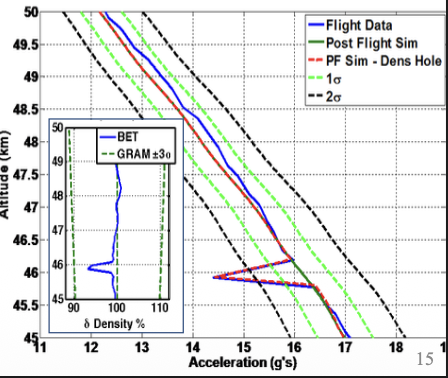
\includegraphics[width=0.7\textwidth]{gambar/accelerationgIRVE3.png}
    \caption{IRVE-3 Post-Flight Simulation vs. Flight Data for Acceleration and Density.}
    \label{fig:irve3_reconstruction}
\end{figure}


\subsection{Trajectory and Heat Rate Scaling}
Comparative analysis of vehicle scale shows that heat rate is a critical function of the nose radius ($R_n$) and vehicle diameter ($D$). As shown in Figure \ref{fig:heatrate_mach}, a smaller 4.572m rigid-body equivalent experiences significantly higher peak heating ($\approx 48 \text{ W/cm}^2$) compared to a 15m inflatable HIAD ($\approx 7 \text{ W/cm}^2$) for the same trajectory~\cite{dillman2015irve3}.

\begin{figure}[H]
    \centering
    \begin{tabular}{cc}
        % First image with caption
        \parbox[c]{0.48\textwidth}{
            \centering
            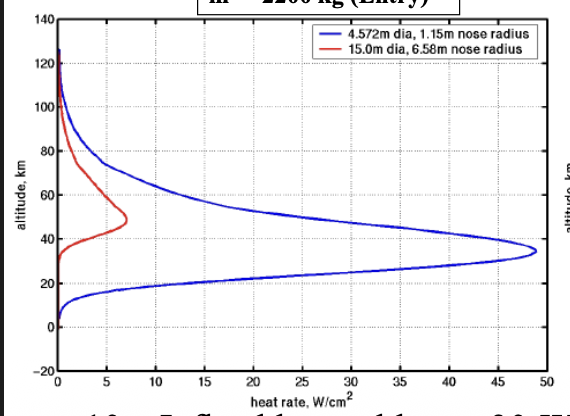
\includegraphics[width=\linewidth]{./gambar/heatratespecirve3.png}
            \captionof{figure}{Heat Rate vs. Altitude}
            \label{fig:heatrate_alt}
        }
        &
        % Second image with caption
        \parbox[c]{0.48\textwidth}{
            \centering
            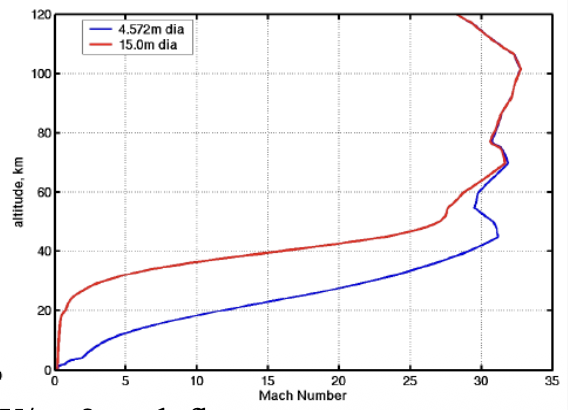
\includegraphics[width=\linewidth]{./gambar/machnumberspecirve3.png}
            \captionof{figure}{Mach Number vs. Altitude}
            \label{fig:mach_alt}
        }
    \end{tabular}
    \caption{Aerothermal scaling comparisons between a 4.57m rigid vehicle and a 15m inflatable HIAD.}
    \label{fig:heatrate_mach}
\end{figure}


\subsection{Conclusions from IRVE-3 Mission Data}
From the available data, several conclusions are drawn to guide the current research:
\begin{enumerate}
    \item \textbf{Scale Benefit:} Increasing the vehicle diameter from a 4.57m rigid capsule to a 15m HIAD reduces peak heating by approximately 85\% due to the increased nose radius ($R_n$), validating the $q \propto 1/\sqrt{R_n}$ relationship.
    \item \textbf{Scalloping Sensitivity:} While large-scale bluntness reduces average heating, IRVE-3 data confirms that the local "scalloped" geometry remains a source of localized heating augmentation that must be resolved via CFD.
    \item \textbf{Atmospheric Uncertainty:} The "density hole" observed at 46 km in IRVE-3 data suggests that real-flight simulations must account for atmospheric variability to accurately predict aerodynamic loads.
\end{enumerate}

\section{Discussion: Synthesis of Hypotheses and Empirical Benchmarks}

The available data from the IRVE-3 and LOFTID missions provide a critical benchmark for validating the hypotheses established in this chapter. By comparing theoretical scaling with flight-test results, the following synthesis is reached:

\subsection{Verification of Scaling and Augmentation Predictions}
The theoretical inverse relationship between heat flux and radius ($q_s \propto 1/\sqrt{R}$) described in Hypothesis 1 is empirically supported by the comparative data between the 4.57m rigid capsule and the 15m HIAD. 
\begin{itemize}
    \item \textbf{Hypothesis Alignment:} The 85\% reduction in heat rate observed when increasing the nose radius validates that the HIAD’s global geometry effectively mitigates aerothermal loads.
    \item \textbf{Scalloping Penalty:} However, the IRVE-3 peak flux of $14.4 \text{ W/cm}^2$ confirms that local "scalloping" can lead to heating levels that exceed smooth-body predictions, necessitating the local high-fidelity CFD resolution proposed in this research.
\end{itemize}

\subsection{Material Safety Margins and Physical Hypotheses}
The hypotheses regarding peak stagnation temperature and heat flux distributions must be viewed within the context of material survival limits.
\begin{itemize}
    \item \textbf{Thermal Buffering:} Hypothesis 2 predicts that valley recirculation will shield the FTPS. This is consistent with IRVE-3 instrumentation data, which showed that internal structure temperatures remained significantly lower than the external flow.
    \item \textbf{Model Fidelity:} The analytical counting of $T_0 = 1320$ K for a calorically perfect gas likely overestimates the temperature compared to the thermally perfect model. Data from the Gen-2 TPS tests ($103 \text{ W/cm}^2$ limit) suggest that the actual heat-sink capacity of the FTPS can handle the predicted high-enthalpy transients, provided that chemical equilibrium effects are correctly modeled.
\end{itemize}

\subsection{Implications for Simulation Strategy}
The "density hole" and acceleration discrepancies found in IRVE-3 post-flight reconstructions highlight the importance of the \textit{Thermally Perfect Gas} and \textit{SST $k-\omega$} models. Standard models failed to fully capture the experimental variations between 45--47 km, supporting the hypothesis that a more sophisticated numerical approach—accounting for variable specific heats and precise boundary layer separation—is required to match real-world flight performance.

\section{Identification of Missing Data and Research Objectives}

While the available data from IRVE-3 and LOFTID provide a foundational understanding of HIAD flight performance, several critical data gaps remain. These gaps define the target of the current research scope and justify the numerical approach proposed in this study.

\subsection{Local Scalloping Effects vs. Global Averages}
The majority of public flight data, such as the IRVE-3 heat rates, provides global or sensor-specific measurements that do not fully resolve the 3D flow field within the toroidal valleys. 
\begin{itemize}
    \item \textbf{Data Gap:} There is a lack of high-fidelity data regarding the \textit{exact} transition point and recirculation dynamics within the "scalloped" gaps at Mach 5 flight conditions.
    \item \textbf{Research Target:} This study aims to fill this gap by providing a detailed 2D axisymmetric map of the pressure and thermal gradients specifically within these toroidal valleys to determine if "dead air" regions effectively shield the FTPS.
\end{itemize}

\subsection{Atmospheric Density Anomalies}
As identified in the IRVE-3 post-flight reconstruction, standard atmospheric models failed to predict the "density hole" and resulting acceleration spikes at 46 km altitude.
\begin{itemize}
    \item \textbf{Data Gap:} Current literature does not sufficiently explain how these localized density variations interact with the complex surface topology of an inflatable decelerator.
    \item \textbf{Research Target:} By utilizing a \textit{Thermally Perfect Gas} model, this research targets the sensitivity of the shock standoff distance and wall heat flux to the real-gas properties that standard calorically perfect models ignore.
\end{itemize}

\subsection{Gen-2 and Gen-3 Material Limits in Scalloped Flow}
While Gen-2 TPS materials have been tested for survival up to $103 \text{ W/cm}^2$ in cold-wall lab conditions, the interaction between these material limits and the heating augmentation caused by surface scalloping is not fully mapped for flight-like profiles.
\begin{itemize}
    \item \textbf{Data Gap:} The quantitative "safety margin" between local heating peaks on toroidal crests and the material thresholds of $400^\circ\text{C}$ is not explicitly established for the mid-entry Mach 5 regime.
    \item \textbf{Research Target:} The primary target of the research scope is to provide a validated comparison between the "Smooth" baseline and the "Scalloped" geometry to quantify the specific heating penalty and assess if it exceeds the thermal limits of current FTPS materials.
\end{itemize}